% Author :  Lionel du Peloux
% Contact : lionel.dupeloux@gmail
% Year : 2017

% ===========================
% COMPILER DIRECTIVES
% ===========================
% !TEX encoding = UTF-8 Unicode
% !TEX TS-program = XeLaTeX-shellescape
% !BIB TS-program = biber
% !BIB program = biber


%%%%%%%%%%%%%%%%%%%%%%%%%%%%%%%%%%%%%%%%%%%%%%%%%%%%%%%%%%%%%%%%%%%%%%%%%%%%%%%%
%%
%% Front Cover
%%
%%%%%

\thispagestyle{empty}
\AddToShipoutPictureBG*{%
	\begin{tikzpicture}[remember picture, overlay, inner sep=0pt]
		\begin{scope}
			\setlength{\pgflinewidth}{0pt}
			\clip (PPbl) rectangle (PPtr);
			\node[anchor=north east] at (PPtr){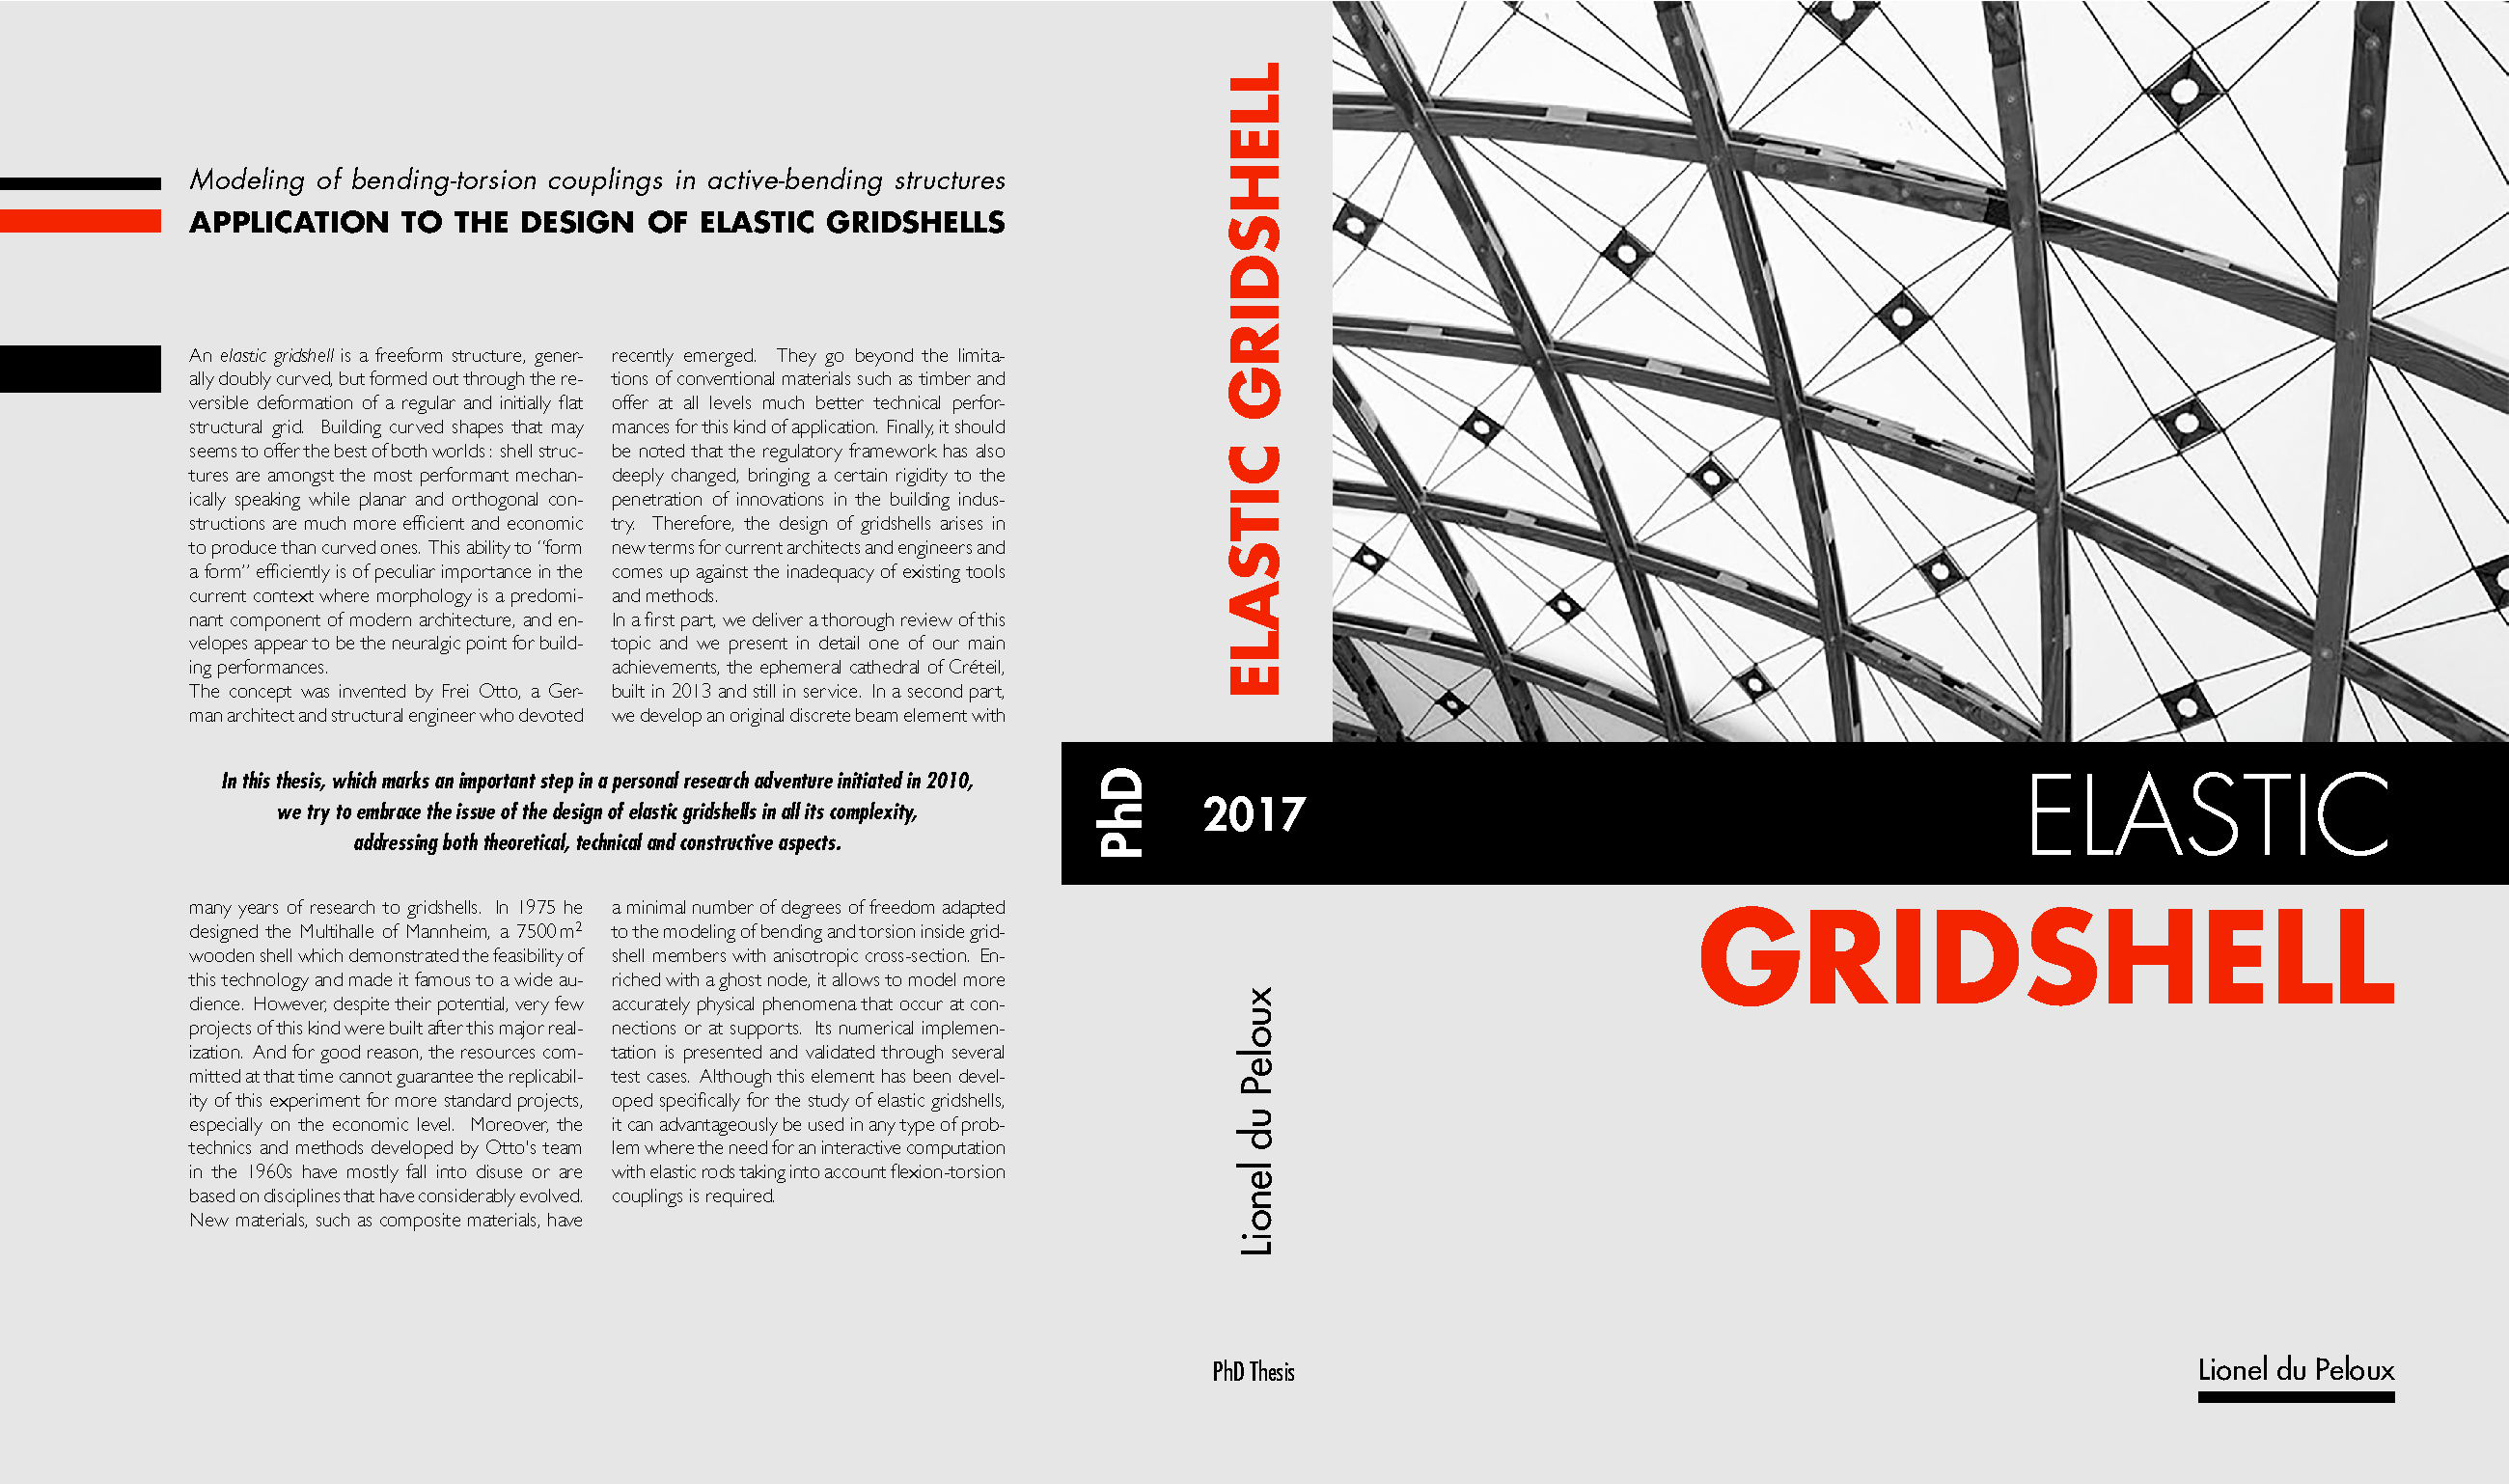
\includegraphics{softcoverwithbleed.pdf}};
		\end{scope}		
	\end{tikzpicture}
}
\hbox{}




%%%%%%%%%%%%%%%%%%%%%%%%%%%%%%%%%%%%%%%%%%%%%%%%%%%%%%%%%%%%%%%%%%%%%%%%%%%%%%%%
%%
%% TITLE PAGE
%%
%%%%%
\clearpage\hbox{}\thispagestyle{empty}
\clearpage\hbox{}\thispagestyle{empty}

% FONT FAMILY
\newfontfamily\FTRegular{FuturaLT}[Scale = MatchUppercase]
\newfontfamily\FTLight{FuturaLT-Light}[Scale = MatchUppercase]
\newfontfamily\FTBold{FuturaLT-Bold}[Scale = MatchUppercase]
\newfontfamily\FTHeavy{FuturaLT-Heavy}[Scale = MatchUppercase]
\newfontfamily\FTBookOblique{FuturaLT-BookOblique}[Scale = MatchUppercase]
\newfontfamily\FTCondensedBoldOblique{FuturaLT-CondensedBoldOblique}[Scale = MatchUppercase]
\newfontfamily\GSLight{GillSans-Light}[Scale = MatchUppercase]
\newfontfamily\FTCondensed{FuturaLT-Condensed}[Scale = MatchUppercase]

% TYPE FACE SECOND FRONT
\DeclareRobustCommand{\tfHA}{\FTBookOblique\fontsize{18pt}{22pt}\selectfont}
\DeclareRobustCommand{\tfHC}{\FTLight\fontsize{15pt}{0pt}\selectfont}
\DeclareRobustCommand{\tfHB}{\FTBold\fontsize{24pt}{30pt}\selectfont}
\DeclareRobustCommand{\tfauthor}{\FTLight\fontsize{14pt}{16pt}\selectfont}
% \sodef\spaceout{}{0pt plus 1fil}{.4em plus 1fil}{0pt}

\begin{tikzpicture}[remember picture, overlay, inner sep=0pt] % ovelay is required, dont now why
	\node[anchor=center] at (PGc){%
		\tfHB
		\fbox{\parbox[c]{0.8\PaperWidth}{%
			\centering
			THE DESIGN OF ELASTIC GRIDSHELLS
	}}};
	\path (PGc) -- (PGt) coordinate[midway] (Pt);
	\node[anchor=center, yshift=0cm] at (Pt){%
		\tfHA%
		\fbox{\parbox[b]{0.8\PaperWidth}{
			\centering
			Modeling of bending-torsion couplings\\ 
			in active-bending structures
	}}};
	\path (PGc) -- (Pt) coordinate[midway] (Pt);
	\node[anchor=center, yshift=0cm] at (Pt){%
		\tfHC%
		\fbox{\parbox[b]{0.8\PaperWidth}{
			\centering
			application to
	}}};
	\node[anchor=south, yshift=1.5cm] at (PGb){%
		\tfauthor%
		\fbox{\parbox[b]{0.8\PaperWidth}{
			\centering
			Lionel du Peloux de Saint Romain\\
			PhD Thesis 2017
	}}};
\end{tikzpicture}




%%%%%%%%%%%%%%%%%%%%%%%%%%%%%%%%%%%%%%%%%%%%%%%%%%%%%%%%%%%%%%%%%%%%%%%%%%%%%%%%
%%
%% MENTIONS
%%
%%%%%
\clearpage\hbox{}\thispagestyle{empty}
\clearpage\hbox{}\thispagestyle{empty}

% TYPE FACE
\DeclareRobustCommand{\tftxt}{\FTBookOblique\fontsize{12pt}{13pt}\selectfont}
\DeclareRobustCommand{\tflabel}{\FTRegular\fontsize{14pt}{0pt}\selectfont}
\DeclareRobustCommand{\tfprenom}{\FTLight\fontsize{14pt}{0pt}\selectfont}
\DeclareRobustCommand{\tfnom}{\FTBold\fontsize{14pt}{0pt}\selectfont}
\newcommand{\nameformat}[2]{\tfprenom #1 \tfnom \MakeUppercase{#2}}

\newlength\HBarTopMargin
\newlength\HBarHeight
\newlength\ColSep
\newlength\LineSkip
\newlength\BigLineSkip

\setlength{\LineSkip}{7mm}
\setlength{\BigLineSkip}{3\LineSkip}
\setlength{\HBarTopMargin}{\BigLineSkip}
\setlength{\HBarHeight}{8mm}
\setlength{\ColSep}{4mm}


\begin{tikzpicture}[remember picture, inner sep=0pt] % ovelay is required, dont now why
	\coordinate[yshift=-\HBarTopMargin] (HBtl) at (PPtl |- PGt);
	\coordinate[yshift=-\HBarHeight] (HBbr) at (HBtl -| PGt);
	\path[fill, secondary] (HBtl) rectangle (HBbr);
	\node[anchor=north east, yshift=-2mm] at (HBbr){%
		\tfHB
		\fbox{\parbox[c]{0.5\PageWidth}{%
			\raggedleft
			\MakeUppercase{These de doctorat}
	}}};
	\coordinate[] (Pt) at (current bounding box.south east);
	\node[anchor=north east, yshift=-6mm] at (Pt){%
		\tftxt
		\fbox{\parbox[c]{0.45\PageWidth}{%
			\raggedleft
			Modeling of bending-torsion couplings in active-\\
			bending structures. Application to the design\\
			of elastic gridshells.
	}}};
	% \filldraw[blue] (HBtl) circle [radius=1mm];
	% \filldraw[blue] (HBbr) circle [radius=1mm];
	% \filldraw[yellow] (current bounding box.south east) circle [radius=1mm];
	% \draw[color=black,thick] (current bounding box.north west) rectangle (current bounding box.south east);
	\pgfresetboundingbox
	\path[use as bounding box] (0,0);
\end{tikzpicture}

\begin{tikzpicture}[remember picture, inner sep=0pt] % ovelay is required, dont now why
	\coordinate[yshift=\BigLineSkip] (Pt) at (PGb);
	\node[anchor=base east] at (Pt){\tflabel\raggedleft Directeur};
	\node[anchor=base west, xshift=\ColSep] at (Pt){\raggedleft \nameformat{Olivier}{Baverel}};
	%
	\coordinate[yshift=\LineSkip] (Pt) at (Pt);
	\node[anchor=base east] at (Pt){\tflabel\raggedleft Invité};
	\node[anchor=base west, xshift=\ColSep] at (Pt){\raggedleft \nameformat{Bernard}{Vaudeville}};
	%
	\coordinate[yshift=\LineSkip] (Pt) at (Pt);
	\node[anchor=base east] at (Pt){\tflabel\raggedleft};
	\node[anchor=base west, xshift=\ColSep] at (Pt){\raggedleft \nameformat{Cyril}{Douthe}};
	%
	\coordinate[yshift=\LineSkip] (Pt) at (Pt);
	\node[anchor=base east] at (Pt){\tflabel\raggedleft};
	\node[anchor=base west, xshift=\ColSep] at (Pt){\raggedleft \nameformat{Jean-François}{Caron}};
	%
	\coordinate[yshift=\LineSkip] (Pt) at (Pt);
	\node[anchor=base east] at (Pt){\tflabel\raggedleft Examinateurs};
	\node[anchor=base west, xshift=\ColSep] at (Pt){\raggedleft \nameformat{Alberto}{Pugnale}};
	%
	\coordinate[yshift=\LineSkip] (Pt) at (Pt);
	\node[anchor=base east] at (Pt){\tflabel\raggedleft};
	\node[anchor=base west, xshift=\ColSep] at (Pt){\raggedleft \nameformat{Carlos}{Lázaro}};
	%
	\coordinate[yshift=\LineSkip] (Pt) at (Pt);
	\node[anchor=base east] at (Pt){\tflabel\raggedleft Rapporteurs};
	\node[anchor=base west, xshift=\ColSep] at (Pt){\raggedleft \nameformat{Sébastien}{Neukirsh}};
	%
	\coordinate[yshift=\LineSkip] (Pt) at (Pt);
	\node[anchor=base east] at (Pt){\tflabel\raggedleft Président};
	\node[anchor=base west, xshift=\ColSep] at (Pt){\raggedleft \nameformat{Bernard}{Maurin}};
	%%
	%%%%%%%
	\coordinate (BXtr) at (current bounding box.north -| PPtr);
	\coordinate (BXbr) at (current bounding box.south -| PGtr);
	\path[black] (current bounding box.north west) rectangle (current bounding box.south east);
	\path[fill, black] (BXtr) rectangle ([xshift=-5\HBarHeight]BXbr);
	%%%%%%%
	%%
	\coordinate[yshift=\BigLineSkip] (Pt) at (Pt);
	\node[anchor=base east] at (Pt){\tflabel\raggedleft Date};
	\node[anchor=base west, xshift=\ColSep] at (Pt){\raggedleft\tfprenom 20 décembre 2017};
	%
	\coordinate[yshift=\LineSkip] (Pt) at (Pt);
	\node[anchor=base east] at (Pt){\tflabel\raggedleft Lieu};
	\node[anchor=base west, xshift=\ColSep] at (Pt){\raggedleft\tfprenom Ecole Nationale des Ponts et Chaussées};
	%
	\coordinate[yshift=\LineSkip] (Pt) at (Pt);
	\node[anchor=base east] at (Pt){\tflabel\raggedleft Auteur};
	\node[anchor=base west, xshift=\ColSep] at (Pt){\raggedleft \nameformat{Lionel}{du Peloux de Saint Romain}};
	%%
	%%
	%%
	\coordinate[yshift=\BigLineSkip] (Pt) at (Pt);
	\node[anchor=base east] at (Pt){\tflabel\raggedleft Spécialité};
	\node[anchor=base west, xshift=\ColSep] at (Pt){\raggedleft\tfprenom Structures et Matériaux};
	%
	\coordinate[yshift=\LineSkip] (Pt) at (Pt);
	\node[anchor=base east] at (Pt){\tflabel\raggedleft Ecole Doctorale};
	\node[anchor=base west, xshift=\ColSep] at (Pt){\raggedleft\tfprenom Science, Ingéniérie et Environnement};
	%
	\coordinate[yshift=\LineSkip] (Pt) at (Pt);
	\node[anchor=base east] at (Pt){\tflabel\raggedleft Laboratoire};
	\node[anchor=base west, xshift=\ColSep] at (Pt){\raggedleft\tfprenom UMR Navier};
	%
	\coordinate[yshift=\LineSkip] (Pt) at (Pt);
	\node[anchor=base east] at (Pt){\tflabel\raggedleft Université};
	\node[anchor=base west, xshift=\ColSep] at (Pt){\raggedleft\tfprenom Paris-Est};
	%
	\pgfresetboundingbox
	\path[use as bounding box] (0,0);
\end{tikzpicture}
